\documentclass[11pt,a4paper]{article}

% --- Packages ---
\usepackage[utf8]{inputenc}
\usepackage[margin=1in]{geometry}
\usepackage{amsmath,amssymb,amsfonts}
\usepackage{graphicx}
\usepackage{booktabs}
\usepackage{tabularx}
\usepackage{hyperref}
\usepackage{listings}
\usepackage{xcolor}
\usepackage{fancyhdr}
\usepackage{tcolorbox}
\usepackage{tikz}
\usetikzlibrary{shapes.geometric, arrows, positioning}

% Define INR symbol fallback
\newcommand{\INR}{\text{INR }}

% --- Color Palette ---
\definecolor{primary}{RGB}{2, 132, 199}
\definecolor{secondary}{RGB}{12, 74, 110}
\definecolor{darkbg}{RGB}{15, 23, 42}
\definecolor{codebg}{RGB}{248, 250, 252}
\definecolor{codeborder}{RGB}{226, 232, 240}
\definecolor{accentgreen}{RGB}{16, 185, 129}
\definecolor{accentred}{RGB}{239, 68, 68}

% --- Hyperref Setup ---
\hypersetup{
    colorlinks=true,
    linkcolor=primary,
    filecolor=magenta,      
    urlcolor=primary,
    pdftitle={Secure Banking Transactions using Digital Signatures},
    pdfpagemode=FullScreen,
}

% --- Listings / Code Block Style ---
\lstdefinestyle{cryptostyle}{
    backgroundcolor=\color{codebg},
    commentstyle=\color{gray},
    keywordstyle=\color{primary}\bfseries,
    numberstyle=\tiny\color{gray},
    stringstyle=\color{accentgreen},
    basicstyle=\ttfamily\footnotesize,
    breakatwhitespace=false,         
    breaklines=true,                 
    captionpos=b,                    
    keepspaces=true,                 
    numbers=left,                    
    numbersep=7pt,                  
    showspaces=false,                
    showstringspaces=false,
    showtabs=false,                  
    tabsize=2,
    frame=single,
    rulecolor=\color{codeborder}
}
\lstset{style=cryptostyle}

% --- Header and Footer ---
\pagestyle{fancy}
\fancyhf{}
\setlength{\headheight}{14pt}
\rhead{\textcolor{gray}{\small Secure Banking with Digital Signatures}}
\lhead{\textcolor{gray}{\small Applied Cryptography}}
\rfoot{\textcolor{gray}{\small Page \thepage}}

\begin{document}

% ==========================================
% TITLE PAGE
% ==========================================
\begin{titlepage}
    \centering
    \vspace*{1.5cm}
    
    {\Huge \bfseries \color{secondary} Secure Banking Transactions\\using Digital Signatures \par}
    \vspace{0.8cm}
    {\Large \textsc{Design, Implementation, and Cryptographic Security Analysis of a Public-Key Authenticated Banking Protocol} \par}
    
    \vspace{1.5cm}
    \rule{\linewidth}{1.5pt}
    \vspace{1.5cm}
    
    \textbf{\Large Applied Cryptography} \\
    \vspace{0.3cm}
    \textsf{Department of Computer Science and Engineering} \\
    \textsf{7th Semester B.Tech Project Report}
    
    \vspace{2.2cm}
    
    \begin{minipage}{0.52\textwidth}
        \begin{flushleft} \large
            \textbf{\color{secondary}Project Members:}\\[0.25cm]
            \begin{tabular}{ll}
                1. Chaitanya & (2306044) \\
                2. Rohith & (2306045) \\
                3. Siddharth & (2306046) \\
                4. Aditya & (2306047) \\
                5. Saim & (2306049) \\
            \end{tabular}
        \end{flushleft}
    \end{minipage}
    \hfill
    \begin{minipage}{0.44\textwidth}
        \begin{flushright} \large
            \textbf{\color{secondary}Course Evaluation:}\\
            \textbf{Academic Year:} 2026--2027\\
            \textbf{Core Modules:}\\
            RSA-2048 Asymmetric Keys\\
            SHA-256 Digest Compression\\
            PKCS\#1 v1.5 Signatures\\
            MITM Attack Interception
        \end{flushright}
    \end{minipage}

    \vfill
\end{titlepage}

\tableofcontents
\newpage

% ==========================================
% SECTION 1: INTRODUCTION
% ==========================================
\section{Introduction}

In modern digital finance, electronic funds transfer (EFT) forms the backbone of global commerce. However, conducting financial transactions over untrusted and open networks (such as the Internet) introduces severe security vulnerabilities, including eavesdropping, message forgery, unauthorized alteration, and replay attacks. 

Traditional symmetric-key systems require both the client and the bank to share a secret key. While efficient, symmetric systems fail to provide non-repudiation and face critical key distribution challenges. To resolve these challenges, public-key asymmetric cryptography combined with cryptographic hash functions is widely adopted.

This project presents an end-to-end, visual, and interactive banking application titled \textbf{``Secure Banking Transactions using Digital Signatures''}. The system implements:
\begin{enumerate}
    \item \textbf{Public-Key Infrastructure (PKI):} Generation and management of 2048-bit RSA key pairs for participating customers.
    \item \textbf{Deterministic Serialization:} Canonical JSON encoding to ensure byte-for-byte consistency across differing client and server platforms.
    \item \textbf{Cryptographic Hashing:} 256-bit SHA-256 message compression to produce fixed-size data fingerprints.
    \item \textbf{Digital Signature Generation:} Client-side encryption of the message digest with the sender's private key under PKCS\#1 v1.5 padding ($S = H^d \pmod n$).
    \item \textbf{Bank-Side Verification:} Mathematical public-key verification by the banking server ($H \stackrel{?}{=} S^e \pmod n$) prior to updating account balances.
    \item \textbf{Man-in-the-Middle (MITM) Interception Simulation:} A dedicated security testing suite demonstrating how in-flight tampering with amounts, beneficiaries, or signature bits triggers immediate mathematical rejection.
\end{enumerate}

% ==========================================
% SECTION 2: THEORETICAL FOUNDATIONS
% ==========================================
\section{Theoretical Foundations}

A secure financial transaction system must enforce the four pillars of information security:
\begin{itemize}
    \item \textbf{Confidentiality:} Ensuring sensitive data cannot be read by unauthorized observers.
    \item \textbf{Integrity:} Ensuring that no part of the message has been altered in transit.
    \item \textbf{Authentication:} Positively confirming the true identity of the transaction originator.
    \item \textbf{Non-Repudiation:} Ensuring that the sender cannot deny having created and transmitted the transfer request.
\end{itemize}

Digital signatures uniquely satisfy \textbf{Integrity}, \textbf{Authentication}, and \textbf{Non-Repudiation} through mathematical guarantees.

\subsection{RSA Key Generation and Mathematical Structure}
The RSA cryptosystem (Rivest–Shamir–Adleman) derives its security from the computational hardness of the \textit{integer factorization problem}. The process consists of three steps:

\begin{enumerate}
    \item Select two large, distinct prime numbers $p$ and $q$.
    \item Compute the RSA modulus:
    \begin{equation}
        n = p \times q
    \end{equation}
    The bit-length of $n$ corresponds to the key length ($2048\text{ bits}$).
    \item Compute Euler's totient function:
    \begin{equation}
        \phi(n) = (p - 1)(q - 1)
    \end{equation}
    \item Choose a public exponent $e$ such that:
    \begin{equation}
        1 < e < \phi(n) \quad \text{and} \quad \gcd(e, \phi(n)) = 1
    \end{equation}
    In this system, $e = 65537$ ($2^{16} + 1$, Fermat prime $F_4$) is selected for optimal modular exponentiation speed and resistance against small-exponent attacks.
    \item Compute the private exponent $d$ using the Extended Euclidean Algorithm:
    \begin{equation}
        d \equiv e^{-1} \pmod{\phi(n)} \iff d \cdot e \equiv 1 \pmod{\phi(n)}
    \end{equation}
    \item Key structures:
    \begin{itemize}
        \item \textbf{Public Key:} $(e, n)$ --- Registered with the Bank PKI Directory.
        \item \textbf{Private Key:} $(d, n)$ --- Kept exclusively on the client's secure local device.
    \end{itemize}
\end{enumerate}

\subsection{Cryptographic Hashing: SHA-256}
Directly signing arbitrary-length transactions via modular exponentiation ($M^d \pmod n$) is computationally prohibitive and algebraically vulnerable to homomorphic multiplicativity attacks. Hence, the \textbf{Hash-then-Sign} paradigm is utilized.

SHA-256 (part of the SHA-2 family defined in FIPS PUB 180-4) operates via the Merkle--Damg{\aa}rd construction on 512-bit message blocks. It satisfies:
\begin{enumerate}
    \item \textbf{Pre-image Resistance (One-Way):} Given $h$, it is computationally infeasible to find $m$ such that $\text{SHA256}(m) = h$.
    \item \textbf{Second Pre-image Resistance:} Given $m_1$, it is infeasible to find $m_2 \neq m_1$ such that $\text{SHA256}(m_1) = \text{SHA256}(m_2)$.
    \item \textbf{Collision Resistance:} It is infeasible to find any pair $m_1 \neq m_2$ yielding identical digests.
    \item \textbf{Avalanche Effect:} Flipping a single bit in the transaction message causes an uncorrelated change in approximately 50\% of the output hash bits.
\end{enumerate}

\subsection{PKCS\#1 v1.5 Digital Signature Scheme}
To prevent mathematical attacks on raw RSA signatures, the SHA-256 hash digest is formatted according to the RSA PKCS\#1 v1.5 standard prior to exponentiation:
\begin{equation}
    \text{EM} = \text{0x00} \parallel \text{0x01} \parallel \text{PS} \parallel \text{0x00} \parallel T
\end{equation}
where:
\begin{itemize}
    \item $\text{PS}$ is an octet string of `0xFF` padding bytes sufficient to make the total encoded length equal to the RSA modulus byte length ($256\text{ bytes}$ for 2048 bits).
    \item $T$ is the DER-encoded \texttt{DigestInfo} structure containing the SHA-256 algorithm Object Identifier (OID: \texttt{2.16.840.1.101.3.4.2.1}) and the 32-byte digest value.
\end{itemize}

The signature integer $s$ is computed as:
\begin{equation}
    s = \text{EM}^d \pmod n
\end{equation}
Upon receiving the signature, the bank server decrypts $s$ using the sender's public exponent $e$:
\begin{equation}
    \text{EM}_{\text{recovered}} = s^e \pmod n
\end{equation}
The bank verifies that $\text{EM}_{\text{recovered}}$ conforms to PKCS\#1 v1.5 format and matches the SHA-256 digest independently computed from the received wire payload.

% ==========================================
% SECTION 3: SYSTEM ARCHITECTURE
% ==========================================
\section{System Architecture and Implementation}

\subsection{User Accounts and Roles}
The banking system is initialized with five registered customer accounts:
\begin{table}[h]
\centering
\small
\begin{tabularx}{\textwidth}{l p{2.8cm} l l r}
\toprule
\textbf{Customer Name} & \textbf{Account Number} & \textbf{Bank Code} & \textbf{Initial Balance} & \textbf{Key Type} \\
\midrule
Siddharth & \texttt{SBIN004829101} & SBI & \INR 85,000.00 & RSA-2048 / SHA-256 \\
Chaitanya & \texttt{HDFC009382102} & HDFC & \INR 62,000.00 & RSA-2048 / SHA-256 \\
Rohith & \texttt{ICIC001920103} & ICICI & \INR 45,000.00 & RSA-2048 / SHA-256 \\
Saim & \texttt{AXIS007182104} & AXIS & \INR 95,000.00 & RSA-2048 / SHA-256 \\
Aditya & \texttt{PNB0003819105} & PNB & \INR 54,000.00 & RSA-2048 / SHA-256 \\
\bottomrule
\end{tabularx}
\caption{System Seed Accounts in SQLite Bank Registry}
\end{table}

\subsection{End-to-End Cryptographic Protocol Workflow}
The workflow is divided into 5 sequential steps:

\begin{figure}[h]
\centering
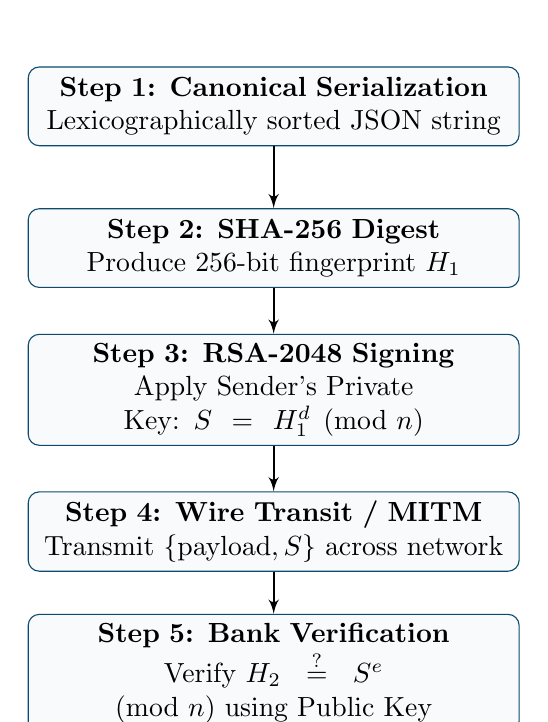
\begin{tikzpicture}[node distance=1.8cm, auto]
    \tikzstyle{block} = [rectangle, draw=secondary, fill=codebg, text width=6cm, text centered, rounded corners, minimum height=1cm]
    \tikzstyle{line} = [draw, -latex', thick]
    
    \node [block] (step1) {\textbf{Step 1: Canonical Serialization}\\Lexicographically sorted JSON string};
    \node [block, below of=step1] (step2) {\textbf{Step 2: SHA-256 Digest}\\Produce 256-bit fingerprint $H_1$};
    \node [block, below of=step2] (step3) {\textbf{Step 3: RSA-2048 Signing}\\Apply Sender's Private Key: $S = H_1^d \pmod n$};
    \node [block, below of=step3] (step4) {\textbf{Step 4: Wire Transit / MITM}\\Transmit $\{ \text{payload}, S \}$ across network};
    \node [block, below of=step4] (step5) {\textbf{Step 5: Bank Verification}\\Verify $H_2 \stackrel{?}{=} S^e \pmod n$ using Public Key};

    \path [line] (step1) -- (step2);
    \path [line] (step2) -- (step3);
    \path [line] (step3) -- (step4);
    \path [line] (step4) -- (step5);
\end{tikzpicture}
\caption{Cryptographic Stepper Protocol Execution Flow}
\end{figure}

\subsection{Core Cryptographic Algorithm Specification}
The signature generation and verification engine operates deterministically according to the following mathematical specifications:

\begin{tcolorbox}[colback=codebg,colframe=codeborder,title=\textbf{Algorithm 1: Client-Side Transaction Signing}]
\textbf{Input:} Transaction Object $\mathcal{P} = \{\text{sender\_acc}, \text{receiver\_acc}, \text{amount}, \text{timestamp}, \text{nonce}\}$, Sender Private Key $K_{\text{priv}} = (d, n)$\\
\textbf{Output:} Base64-encoded Digital Signature $S$
\begin{enumerate}
    \item \textbf{Canonical Serialization:} Convert $\mathcal{P}$ into a deterministic byte stream $\mathcal{M}$ by sorting all JSON keys in ascending lexicographical order:
    \begin{equation}
        \mathcal{M} \leftarrow \text{CanonicalEncode}(\mathcal{P})
    \end{equation}
    \item \textbf{Cryptographic Hashing:} Compute the 256-bit message digest using SHA-256:
    \begin{equation}
        H \leftarrow \text{SHA-256}(\mathcal{M})
    \end{equation}
    \item \textbf{PKCS\#1 v1.5 Formatting:} Encode digest $H$ with DER-encoded \texttt{DigestInfo} and \texttt{0xFF} padding string $\text{PS}$:
    \begin{equation}
        \text{EM} \leftarrow \text{0x00} \parallel \text{0x01} \parallel \text{PS} \parallel \text{0x00} \parallel \text{DigestInfo}(H)
    \end{equation}
    \item \textbf{Modular Exponentiation:} Sign the formatted digest using sender's private exponent $d$:
    \begin{equation}
        S \leftarrow \text{EM}^d \pmod n
    \end{equation}
    \item \textbf{Return:} Output digital signature $S$ formatted as a base64 octet string.
\end{enumerate}
\end{tcolorbox}

\begin{tcolorbox}[colback=codebg,colframe=codeborder,title=\textbf{Algorithm 2: Bank-Side Signature Verification}]
\textbf{Input:} Received Wire Payload $\mathcal{P}_{\text{wire}}$, Digital Signature $S$, Sender Public Key $K_{\text{pub}} = (e, n)$\\
\textbf{Output:} Boolean verdict $\in \{\textbf{True}, \textbf{False}\}$
\begin{enumerate}
    \item \textbf{Recompute Hash:} Derive canonical representation $\mathcal{M}_{\text{wire}} = \text{CanonicalEncode}(\mathcal{P}_{\text{wire}})$ and compute:
    \begin{equation}
        H_{\text{recomputed}} \leftarrow \text{SHA-256}(\mathcal{M}_{\text{wire}})
    \end{equation}
    \item \textbf{Public-Key Decryption:} Decrypt signature $S$ using registered public exponent $e$:
    \begin{equation}
        \text{EM}_{\text{recovered}} \leftarrow S^e \pmod n
    \end{equation}
    \item \textbf{Verification \& Equality Check:} Extract recovered hash $H_{\text{extracted}}$ from $\text{EM}_{\text{recovered}}$. If the structure conforms to PKCS\#1 v1.5 and:
    \begin{equation}
        H_{\text{recomputed}} == H_{\text{extracted}}
    \end{equation}
    then return \textbf{True} (Authentic \& Intact); otherwise, return \textbf{False} (Tampered / Forged).
\end{enumerate}
\end{tcolorbox}

% ==========================================
% SECTION 4: SECURITY ANALYSIS & MITM
% ==========================================
\section{Security Analysis \& Attack Simulation}

\subsection{Man-in-the-Middle (MITM) Tampering Scenarios}
To empirically test and prove the security properties of digital signatures, the application includes a live MITM Interceptor console that executes three attack vectors:

\begin{enumerate}
    \item \textbf{Scenario 1: Amount Tampering}
    \begin{itemize}
        \item \textit{Attack Action:} Siddharth initiates a transfer of \INR 2,500 to Chaitanya. An active adversary intercepts the unencrypted wire packet and alters the amount to \INR 30,000.
        \item \textit{Detection Mechanism:} The bank receives the tampered amount and recomputes the SHA-256 hash $H_2$. Because of the avalanche effect, $H_2$ differs from the client-signed hash $H_1$.
        \item \textit{Outcome:} \texttt{ERR\_SIGNATURE\_MISMATCH}. The bank server identifies that $H_2 \neq S^e \pmod n$, aborts the transfer, logs the security event, and prevents fund loss.
    \end{itemize}

    \item \textbf{Scenario 2: Beneficiary Diversion (Receiver Spoofing)}
    \begin{itemize}
        \item \textit{Attack Action:} The adversary substitutes Chaitanya's legitimate account number (\texttt{HDFC009382102}) with an attacker-controlled account (\texttt{HACK999999999}).
        \item \textit{Outcome:} Changing the receiver string alters the canonical byte stream, breaking hash equivalence. The signature is mathematically rejected.
    \end{itemize}

    \item \textbf{Scenario 3: Signature Byte Corruption}
    \begin{itemize}
        \item \textit{Attack Action:} The adversary modifies several characters in the base64 signature block or attempts to forge a signature without possessing Siddharth's private key.
        \item \textit{Outcome:} Decryption under Siddharth's public key fails to decode valid PKCS\#1 v1.5 padding. The verifier returns \texttt{false}.
    \end{itemize}
\end{enumerate}

\subsection{Replay Attack Mitigation (Cryptographic Nonce)}
If an eavesdropper records a valid wire packet $\{ \text{payload}, S \}$ and transmits it repeatedly to drain the sender's balance, digital signatures alone cannot detect the duplicate because the signature is mathematically valid. 

To counteract this, the system embeds:
\begin{enumerate}
    \item A high-entropy, single-use cryptographic \textbf{nonce} (e.g., \texttt{NONCE-7F3A92B1}).
    \item A millisecond UNIX \textbf{timestamp}.
\end{enumerate}
The bank maintains an indexed cache $\mathcal{N}_{\text{processed}}$ of all previously executed nonces. Upon receiving a transfer request containing nonce $\eta$ from user $U_i$, the server verifies state membership:
\begin{equation}
    \eta \notin \mathcal{N}_{\text{processed}}(U_i)
\end{equation}
If $\eta \in \mathcal{N}_{\text{processed}}(U_i)$, the transaction is flagged as a duplicate replay attack and rejected immediately:
\begin{tcolorbox}[colback=accentred!10!white,colframe=accentred,title=\textbf{Replay Attack Detected}]
\texttt{REJECTED\_REPLAY\_ATTACK: Cryptographic Nonce previously used. Transaction aborted.}
\end{tcolorbox}
Otherwise, $\eta$ is atomically inserted into $\mathcal{N}_{\text{processed}}(U_i)$ before transaction settlement.

% ==========================================
% SECTION 5: EXPERIMENTAL RESULTS
% ==========================================
\section{Experimental Results and Verification}

\subsection{Test Case 1: Legitimate Signed Transaction}
\begin{itemize}
    \item \textbf{Sender:} Siddharth (\texttt{SBIN004829101})
    \item \textbf{Beneficiary:} Saim (\texttt{AXIS007182104})
    \item \textbf{Amount:} \INR 5,000.00
    \item \textbf{Nonce:} \texttt{NONCE-8X19B4C2}
    \item \textbf{Client Hash ($H_1$):} \texttt{a9f81d4b6807f43c... (64 hex characters)}
    \item \textbf{Signature ($S$):} 2048-bit base64 block generated using Siddharth's private key.
    \item \textbf{Server Verification Result:}
    \begin{itemize}
        \item $H_1 == H_2$: \textbf{TRUE (MATCH)}
        \item Verdict: \textbf{SETTLED\_VERIFIED}
        \item Balance Update: Siddharth \INR 85,000 $\to$ \INR 80,000; Saim \INR 95,000 $\to$ \INR 100,000.
    \end{itemize}
\end{itemize}

\subsection{Test Case 2: Tampered Wire Packet (Amount Alteration)}
\begin{itemize}
    \item \textbf{Sender:} Siddharth
    \item \textbf{Beneficiary:} Chaitanya
    \item \textbf{Original Amount:} \INR 2,500.00 $\longrightarrow$ \textbf{In-Flight Altered Amount:} \INR 30,000.00
    \item \textbf{Client Hash ($H_1$):} \texttt{c4819d7a220e8910...}
    \item \textbf{Server Recomputed Hash ($H_2$):} \texttt{f024be51aa76391d...}
    \item \textbf{Comparison:} $H_1 \neq H_2$ (64 out of 64 hex characters altered).
    \item \textbf{Server Verification Result:}
    \begin{itemize}
        \item Verdict: \textbf{REJECTED\_SIGNATURE\_MISMATCH}
        \item Account Balances: Unchanged (Zero fund loss).
    \end{itemize}
\end{itemize}

% ==========================================
% SECTION 6: CONCLUSION
% ==========================================
\section{Conclusion}

The project \textbf{``Secure Banking Transactions using Digital Signatures''} demonstrates the practical application of modern public-key cryptography in protecting financial transactions. Through the synergy of:
\begin{itemize}
    \item \textbf{RSA-2048} asymmetric key pairs for mathematical identity binding,
    \item \textbf{SHA-256} for one-way message compression and collision resistance,
    \item \textbf{PKCS\#1 v1.5} encoding to eliminate mathematical vulnerabilities, and
    \item \textbf{Cryptographic Nonces} to neutralize replay attacks,
\end{itemize}
the system guarantees that no financial payload can be intercepted, forged, or altered in transit without detection by the banking server. The interactive 5-step stepper and MITM attack console provide an intuitive demonstration of cryptographic security in action.

% ==========================================
% REFERENCES
% ==========================================
\begin{thebibliography}{99}
\bibitem{rsa} R. L. Rivest, A. Shamir, and L. Adleman, ``A Method for Obtaining Digital Signatures and Public-Key Cryptosystems,'' \textit{Communications of the ACM}, vol. 21, no. 2, pp. 120--126, 1978.
\bibitem{fips180} National Institute of Standards and Technology (NIST), ``Secure Hash Standard (SHS),'' \textit{Federal Information Processing Standards Publication (FIPS PUB) 180-4}, 2015.
\bibitem{pkcs1} J. Jonsson and B. Kaliski, ``Public-Key Cryptography Standards (PKCS) \#1: RSA Cryptography Specifications Version 2.1,'' \textit{RFC 3447}, 2003.
\bibitem{stallings} W. Stallings, \textit{Cryptography and Network Security: Principles and Practice}, 8th ed., Pearson, 2020.
\end{thebibliography}

\end{document}

